\chapter{Testing}
There are two main ways to make sure that a web application works properly and fulfills it's role. On one hand there is a code performance testing, performing test on backend level with dummy data insertion and performance benchmarking. On the other hand there is testing to assure that users are able to use system and to get inspiration for future ux iterations via SUS.
\section{Performance testing}
Performance script \textbf{dummy\_data\_benchmark.php} \footnote{In https://github.com/KlosStepan/SwimmPair-Www \textbf{dummy\_data\_benchmark.php}} is located in main swimmpair folder. It is performed on default database installation (w/ 2 admin users, w/ already existing clubs administered by application requesters, and default referee positions).  
\newline
\textbf{The script has several tasks (tests) which are performed and benchmarked.}
\begin{enumerate}
    \item \underline{Create 98 Users} (no. 3-100) - each random affiliation to existing Club (no. 1-15).
    \item \underline{Create 12 Cups} - each random affiliation to existing Club (no. 1-15).
    \item \underline{Fetch new Users}, \underline{fetch new Cups} (+ \underline{fetch static Positions}).
    \item \underline{Create Availabilities} (20 Users available per Cup).
    \item \underline{Create Pairings} (each Availability gets 1 random position).
    \item \underline{Call stats queries} (20 - randomly either Clubs or Users stats w/ random club\_id or user\_id).
\end{enumerate}
\textbf{Docker Compose} - 2.3 GHz Core i5 (I5-8259U) RAM 16GB Storage 512GB
\newline
\begin{tabular}{ |c|c|c|c|c|c|c|c|c|c|c|c| } 
    \hline
    T/rep no. & \#1 & \#2& \#3& \#4& \#5& \#6& \#7& \#8& \#9& \#10 \\
    \hline
    Test \#1 & 7.02 & 7.04& 6.61& 7.89& 6.73& 6.62& 6.66& 7.34& 7.19& 6.54 \\ 
    Test \#2 & 0.08 & 0.06& 0.06& 0.06& 0.06& 0.10& 0.58& 0.60& 0.50& 0.15 \\ 
    Test \#3 & 7.02 & 7.05& 6.61& 7.90& 6.74& 6.63& 6.66& 7.35& 7.20& 6.55 \\ 
    Test \#4 & 1.24 & 1.05& 1.14& 1.05& 1.18& 1.17& 1.24& 1.15& 0.96& 1.59 \\ 
    Test \#5 & 8.02 & 7.87& 7.39& 8.95& 7.70& 7.81& 7.44& 8.12& 7.98& 7.36 \\ 
    Test \#6 & 1.29 & 1.10& 1.19& 1.12& 1.23& 1.22& 1.28& 1.19& 1.00& 1.62 \\ 
    TOTAL & \underline{9.31} & \underline{8.97}& \underline{8.59}&\underline{10.06}& \underline{8.93}& \underline{9.03}& \underline{8.72}& \underline{9.31}& \underline{8.98}& \underline{8.98} \\ 
    \hline
\end{tabular}
\newline
\textbf{Kubernetes} - \textbf{DOKS} Kubernetes v 1.25.4-do.0, \textbf{2x Node} s-1vcpu-2gb-intel
\newline
\begin{tabular}{ |c|c|c|c|c|c|c|c|c|c|c|c| } 
    \hline
    T/rep no. & \#1 & \#2& \#3& \#4& \#5& \#6& \#7& \#8& \#9& \#10 \\
    \hline
    Test \#1 & 7.08 & 6.87& 6.79& 6.85& 7.20& 7.10& 6.77& 6.85& 6.81& 6.79 \\ 
    Test \#2 & 0.04 & 0.03& 0.04& 0.04& 0.04& 0.03& 0.05& 0.05& 0.03& 0.04 \\ 
    Test \#3 & 7.08 & 6.88& 6.79& 6.86& 7.20& 7.10& 6.77& 6.85& 6.81& 6.79 \\ 
    Test \#4 & 0.84 & 0.59& 0.68& 0.81& 0.60& 0.55& 0.70& 0.82& 0.60& 0.67 \\ 
    Test \#5 & 7.72 & 7.40& 7.55& 7.56& 7.69& 7.60& 7.35& 7.56& 7.33& 7.40 \\ 
    Test \#6 & 0.86 & 0.61& 0.70& 0.84& 0.62& 0.57& 0.72& 0.84& 0.62& 0.69 \\ 
    TOTAL & \underline{8.57} & \underline{8.01}& \underline{8.25}& \underline{8.40}& \underline{8.31}& \underline{8.17}& \underline{8.07}& \underline{8.39}& \underline{7.95}& \underline{8.09} \\ 
    \hline
\end{tabular}
\section{User testing}
We carried on testing of our application by handing SUS questionare to 20 respondents. We then evaluated the scores in order to find out how our application stands. These people are are either managers or common referees \footnote{\cite{SUSDesc}}. 
\newline
\textbf{Questionare is made of 10 questions scored 1-5.}
\begin{enumerate}
    \item I think that I would like to use this system frequently.
    \item I found the system unnecessarily complex.
    \item I thought the system was easy to use.
    \item I think that I would need the support of a technical person to be able to use this system.
    \item I found the various functions in this system were well integrated.
    \item I thought there was too much inconsistency in this system.
    \item I would imagine that most people would learn to use this system very quickly.
    \item I found the system very cumbersome to use.
    \item I felt very confident using the system.
    \item I needed to learn a lot of things before I could get going with this system.
\end{enumerate}
\textbf{We collected SUS feedbacks from 20 people using our system.}\footnote{((A1-1)+(5-A2)+(A3-1)+(5-A4)+(A5-1)+(5-A6)+(A7-1)+(5-A8)+(A9-1)+(5-A10))*2,5}
\newline
\begin{tabular}{ |c|c|c|c|c|c|c|c|c|c|c|c| } 
    \hline
    Respondent / Q. no. & \#1 & \#2& \#3& \#4& \#5& \#6& \#7& \#8& \#9& \#10 \\
    \hline
    Petr A - \textbf{87.5}     & 5 & 1& 3& 1& 5& 1& 3& 1& 5& 2 \\ 
    Olga A - \textbf{72.5}     & 2 & 1& 3& 2& 4& 1& 5& 1& 3& 3 \\ 
    Marin H - \textbf{75}    & 3 & 1& 4& 2& 5& 1& 3& 2& 3& 2 \\ 
    Michaela H - \textbf{60} & 2 & 3& 3& 4& 3& 2& 4& 2& 5& 2 \\ 
    Stepan K - \textbf{85}   & 5 & 2& 4& 1& 3& 1& 3& 1& 5& 1 \\ 
    Matylda K - \textbf{80}  & 4 & 1& 4& 2& 4& 1& 4& 2& 4& 2 \\ 
    Lukas Kour. - \textbf{67.5} & 2 & 2& 5& 2& 4& 1& 4& 2& 2& 3 \\ 
    Jana K - \textbf{60}    & 1 & 2& 3& 2& 5& 2& 3& 2& 2& 2 \\ 
    Lukas Kous. - \textbf{92.5} & 5 & 1& 4& 1& 5& 1& 4& 1& 5& 2 \\ 
    Zuzana K - \textbf{70}   & 3 & 2& 5& 1& 3& 1& 3& 2& 3& 3 \\ 
    Eva K - \textbf{80}      & 3 & 2& 5& 1& 3& 1& 3& 1& 4& 1 \\ 
    Michael P - \textbf{75}  & 2 & 1& 4& 3& 4& 1& 4& 1& 3& 1 \\ 
    Lenka P - \textbf{70}    & 3 & 2& 5& 1& 3& 2& 3& 2& 3& 2 \\ 
    Daniela S - \textbf{77.5}  & 3 & 2& 5& 2& 3& 1& 4& 2& 4& 1 \\ 
    Magdalena S - \textbf{85} & 4 & 1& 4& 1& 4& 1& 5& 1& 3& 2 \\ 
    Jiri S - \textbf{62.5}     & 3 & 3& 5& 3& 4& 2& 3& 3& 2& 1 \\ 
    Hana S - \textbf{80}     & 2 & 2& 4& 1& 5& 1& 4& 1& 4& 2 \\ 
    Alena T - \textbf{90}    & 4 & 1& 5& 1& 3& 1& 4& 1& 5& 1 \\ 
    Magda Z - \textbf{85}    & 3 & 2& 5& 2& 4& 1& 4& 1& 5& 1 \\ 
    Vera Z - \textbf{75}     & 3 & 3& 4& 1& 3& 1& 3& 1& 4& 1 \\ 
    \hline
\end{tabular}
\newpage
Rest of this stuff mby \textbf{depr.}
\begin{lstlisting}
//1. Create 98 Users - random affil to 1-15
$usersManager->RegisterUser($first_name, $last_name, $email, 12345, $rights[$rights_idx], $ranks[$rrid_idx]->id, $clubs[$club_idx]->id);
//2. Create 12 Cups
$cupsManager->InsertNewCup($cups_names[$cup_name_idx]." ".rand(1, 8), "2023-".str_pad($j, 2, '0', STR_PAD_LEFT)."-26", "2023-".str_pad($j, 2, '0', STR_PAD_LEFT)."-28", $clubs[$club_idx]->id, $content[$content_idx]);
//3. Fetch new Users and Cups (&positions)
$users = $usersManager->FindAllActiveUsersOrderByLastNameAsc();
$cups = $cupsManager->FindAllUpcomingCupsEarliestFirst();
$positions = $positionsManager->FindAllPositions();
//4. Create Availabilities
$cupsManager->InsertNewAvailability($cups[$k]->id, $users[$user_idx[$kk]]->id, 1);
//5. Create Pairings (availabilities 1 random pos. for each)
$cupsManager->InsertNewPairing(($l+1), $positions[$position_idx]->id, $avails[$ll]->id);
echo("6. Call stats queries (20 either Clubs/Users stat queryings)<br/>\r\n");
$personCupsCount = $usersManager->CountCupsAttendanceOfUserGivenYear($users[$user_idx]->id, $year);
$stats_cups = $usersManager->CountOverallStatisticsOfUserGivenYear($users[$user_idx]->id, $year);
$stats_users = $usersManager->CountClubSeasonalStatistics($clubs[$club_idx]->id, $year);
\end{lstlisting}
This benchmark snippet probably \textbf{depr.}
\newline
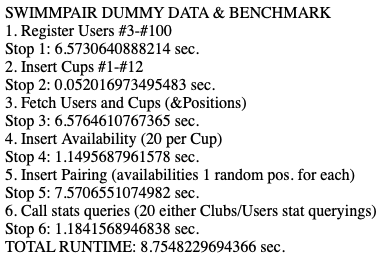
\includegraphics[scale=0.707]{img/app-benchmarking.png}